\documentclass[a4paper,12pt]{article}

\usepackage[utf8]{inputenc}
\usepackage{geometry}

\geometry{
    left=1cm,
    right=1cm,
    top=1.5cm,
    bottom=2.5cm
}

\usepackage{setspace}
\usepackage{tikz}
\usepackage{tkz-graph}
\usetikzlibrary{trees}

\definecolor{lightblue}{RGB}{182, 249, 255}
\definecolor{darkblue}{RGB}{19, 75, 95}
\definecolor{bluedot}{RGB}{81,171,203}

\begin{document}
 
\pagenumbering{arabic}

\begin{Large}
    \begin{singlespace}
       \begin{center}
        \textbf{Queue - Template} \\
        Version 1.0.0
       \end{center} 
    \end{singlespace}
\end{Large}

\vspace*{10mm}

\begin{center}
    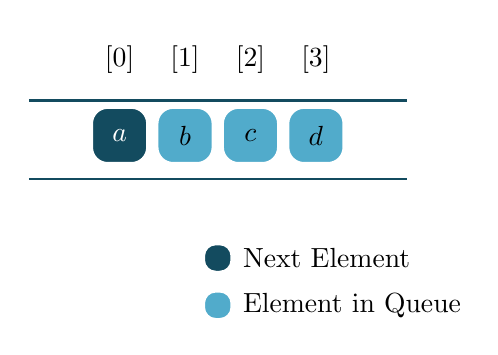
\begin{tikzpicture}[thick, 
        main/.style = {draw=white, text=black, fill=bluedot,rounded corners=2mm,minimum size=2em}, scale=0.2,
        selected/.style = {draw=white, text=white, fill=darkblue,rounded corners=2mm,minimum size=2em},
        EdgeStyle/.append style = {->, draw=darkblue, thick}]
        \matrix [column sep=0.1cm, row sep=0.3cm]{
        \node[] (1) {$[0]$}; & \node[] (3) {$[1]$}; & \node[] (5) {$[2]$}; & \node[] (7) {$[3]$}; \\
        \node[selected] (2) {$a$}; & \node[main] (4) {$b$}; & \node[main] (6) {$c$}; & \node[main] (8) {$d$}; \\ 
    };
    \draw[draw=darkblue] (-12,0) -- (12, 0);
    \draw[draw=darkblue] (-12,-5) -- (12, -5);

    \node[draw=white, text=white, fill=darkblue,rounded corners=1.5mm,minimum size=1em,label=right:Next Element] (A) at (0,-10) {};
    \node[draw=white, text=white, fill=bluedot,rounded corners=1.5mm,minimum size=1em,label=right:Element in Queue] (A) at (0,-13) {};
    \end{tikzpicture}
\end{center}
    
\end{document}